\chapter[Opportunities For Interventions][]{Opportunities For Interventions: Making the Field More Equitable}

\section{Preamble}

\section{Introduction}


\begin{figure}[ht]
\centering
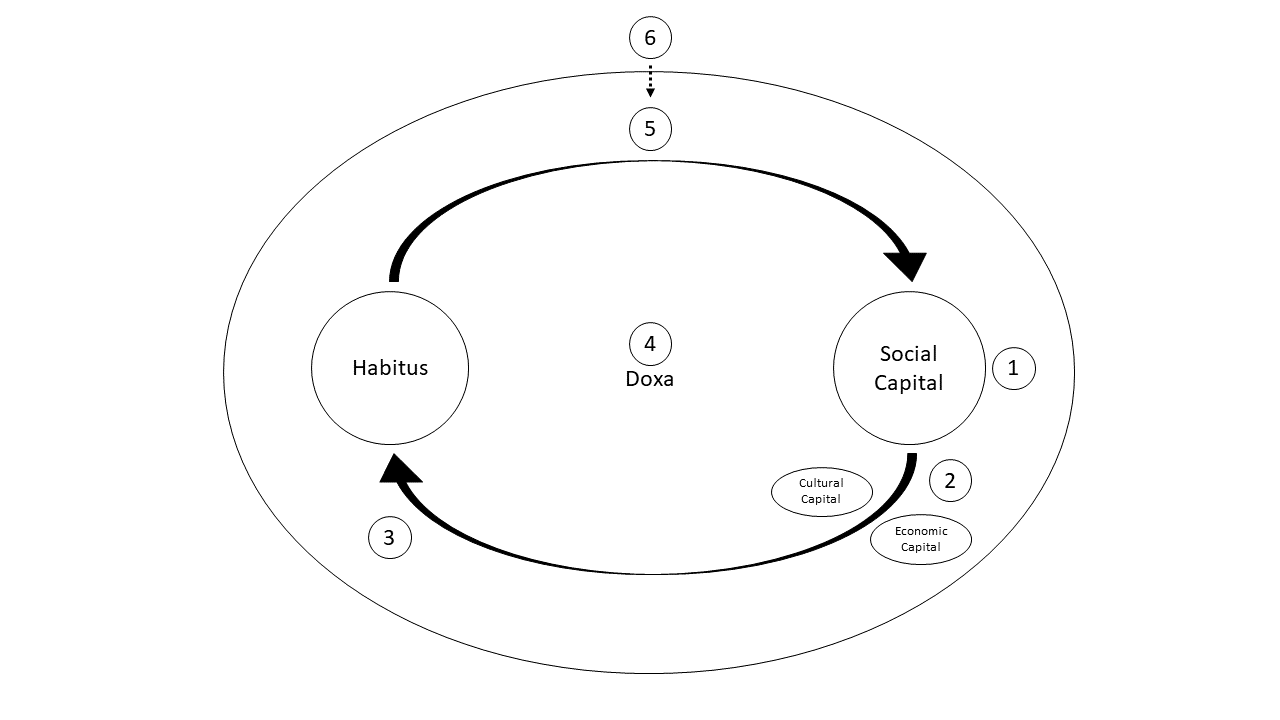
\includegraphics[width=\textwidth]{C5 - Understanding Capital Accumulation/HabitusSocCap_TheoreticalModel.png}
\caption{\label{fig:HabitusSocCap_TheoreticalModel_C7}\textbf{Complete Theoretical Model}. The complete theoretical model. The model, informed by the described experiences of university science students, expands on the interaction between habitus and capital originally illustrated by \cite{Bourdieu1984}. The model provides a step by step description of how social capital translates into habitus transformation, and how habitus generates future capital accumulation. Step 1 refers to the initial availability of social capital for an individual. Step 2 refers to the value gained through leveraging social capital into forms of economic and cultural capital. Step 3 refers to how social capital is internalised by the individual. Step 4 refers to how habitus informs the acquisition of future social capital. 5 refers to factors outside of the individual that structure the field (by availability of capital and exchange value).}
\end{figure}

\section{Social Capital in the Field of University Science (Step 1)}
This section discusses the availability of social relationships that participants had in the field of university science. These relationships are categorised into three key groups, social capital through family connections, social capital through lecturers, and social capital through peers. 

\subsection{Prior to University: Increase Availability of Connections}
It may be possible to address equity issues by increasing the availability of these relationships to students who would not have access to them in their everyday life. Interventions, provided by institutional support services or groups outside of institutions, can mobilise structural changes in the field by increasing the availability of connections. For participants in the current study, those who held connections with people who had careers in science (e.g., family members, friends, mentors, lecturers) or experience of university appeared to be the most at home at university. Students who do not have access to these forms of social capital may struggle to envision different careers in science, and what is required to progress in the field. While tertiary-based programmes such as science scholars can boost the social capital of students who have already demonstrated some success in science, it is also important to target students at earlier stages before deficits in social capital have detrimental impacts on students' educational trajectories. As Patrick argued: ``If I just got someone to talk to me when I was young to get me interested in computer science I think that would help.''   


\subsection{For University}
Support services can provide physical spaces that can help students facilitate connections. Patrick, who entered university without much peer support, met most of his friends through Tuakana, while Sean, a member of the MAPAS programme was able to connect with other students who also hung out at the MAPAS house. Mark highlighted how being in the same physical space as other students outside of the classroom may have helped him seek out advice when he would not have sought it otherwise: \blockquote{since I’m staying at halls there are lots of engineers within my own floor... if we are in the common room we can all get together and kind of support each other in that way and people will ask each other concepts and how they do things and people can explain it through like that. So I think that is pretty beneficial towards me because having to actively search out when I need help is something that I am going to have to adjust to, but having that just right there means that I can easily join in and just pull out my laptop and take down some notes or help with certain things.}


Support initiatives may also help increase students social capital when it comes to finding employment. For example, Belvia noted how a Women in Computer Science group could aid her in getting her CV out to companies. Many of the participants in the current study gained information about prospective fields through university open days, with this commonly being cited as an important influence in sparking aspirations. 





\section{Leveraging Social Capital (Step 2)}
The value of social capital is derived from the economic and cultural capital that can be mobilised through connections with others. These resources may provide students with advantages in supporting their learning and providing student access to information about the field. 

\subsection{Prior to University:: Equitable Resourcing for Educational Institutions}

Students are more likely to leverage the value of their social relationships with teachers if the teacher is supported in their classroom. The funding available to schools can impact on the teaching resources that teachers can draw upon, and also the structure of the classroom itself. 

The experiences of participants revealed how science is taught in schools can differ greatly one one school to the next. While some participants recalled how their learning focused on learning from textbooks, other participants were given opportunities to engage with more hands-on activities. Participants noticed how inequities in resourcing resulted in very different learning experiences. After moving from a private school to a low decile rural school, Stephen felt science lessons were less engaging: \blockquote{we are quite a low decile school, so we didn't have the resources I guess to make it fun because I was getting all these on like Snapchat all these Private School people were like posting all these cool things they were doing at science and I'm here, teacher just teach me stuff on the whiteboard}.  


Resourcing may be a contributing factor to classroom size, which can impact on learning outcomes. Lily experienced a different class environment when her teachers were managing smaller classes: \blockquote{teachers got a bit more enthusiastic about teaching our Year 13 classes rather than when they had to teach like Year 9 and 10 classes before NCEA or even the first level 1 NCEA classes they were a lot less enthusiastic about just because like I say a lot of people were there just to muck around.}. Belvia felt being in a small class gave her more opportunity ``to get close to the teacher and ask them questions'', while it was more difficult in bigger classes: \blockquote{it felt like closer it was much more easier to ask any questions. I could put my hand up and ask her to come, but in chemistry I feel like it was too many more people, it was like far away I will just ask him and he's busy sorry when he's free.} Class size may be a constraint for teachers, even when they demonstrate good pedagogy. \blockquote{I guess more one on one time would have been nice, but with a class of 30 you can’t really ask that much more, but they were just really interactive with their students.} Highly resourced schools may be more able to provide students with learning opportunities that cater to individual needs. Susan, who went to a high decile private school , described how her school created a new advanced class for herself and two other students: \blockquote{They created our own class for us, which was taught by the physics and the chemistry teacher. [They] would alternate with us and we would focus on scholarships and also do the rest of the internals.
} In contrast, Stephen's high school classes tended to contain a mixture of students studying different standard levels: \blockquote{When you are lost and you are stuck you couldn't really go up to them [teachers] because in my English class we had like 25 students, but obviously the majority of them were level 2. So we had to kind of mix it in and the teacher had to keep going back and forth between the levels and it was kind of stressful for her, but besides that it was fun except for the fact we had a bunch of level 2 people in our class and we couldn't really do it to our own standard.
} Stephen's recollection also points to the increased strain the increased classroom size of mixed ability students can have on the teacher. 

\subsection{For University: Preparatory Courses}
Students may enter university with gaps in their knowledge, unwittingly or otherwise. Some participants noticed gaps in their learning once they transitioned to university study. In these cases, foundation courses may be particularly helpful in bringing students up to the standard needed for future university courses. Lily took part in the Hikitia Te Ora course, which aimed to help her cover gaps in physics, chemistry and biology coming into university. While Lily did not have those gaps, she recognised the benefits of Hikitia Te Ora in helping her adapt to a new lifestyle: \blockquote{I didn't have those gaps, but it was more of a transition in terms of confidence for me. Like coming into university I knew it would be a different lifestyle, a different format of studying and all that sort of thing.}


\section{Internalising Capital (Step 3)}
The capital that students accrue in university science not only provides access to resources, but it can also influences the way that students see themselves in the field. Capital, which determines students position in the field, is internalised by students via their habitus, which establishes the students disposition towards the field \cite{Bourdieu1992}. Students who hold high levels of social capital may feel an affinity with the field and see progression to university as a path already drawn out. While some participants found developing relationships with those with power in the field normal, others participants did not make full use of connections as they found it ``nerve-wracking'', their lecturers ``distant'' or intimidating. 

\subsection{Prior to University:}

\subsection{For University: Educator Service Training}
Support services can facilitate students' development of social capital by providing learning environments that are welcoming. This is particularly important in classroom settings, where poor pedagogy can reduce student engagement with course content or cause students to  drop out of courses \cite{russell2011factors}. Efforts to train university teachers can improve student outcomes \cite{gibbs2004impact}, while research from New Zealand suggests that improving the cultural competence of teachers may be especially important for students who are from marginalised groups \cite{ikiua2019pasifika} and/or have English as a second language \cite{campbell2008asian}. Reframing the student-teacher relationship so it is more student-focused \cite{gibbs2004impact} and culturally responsive \cite{ikiua2019pasifika} may reduce the ``distance'' felt by students learning science at university.  

research points to the importance of culturally responsive pedagogies \citep{glynn2010culturally}


\section{Doxa (Step 4)}
Outside of the of the social relationships that students hold, general discourses in society influence the development of habitus. As identified in Chapter 6, participants recalled experiences of dealing with stereotypes operating in the fields of education, science, and university. University also tends to be viewed as a context with a heightened focus on independent learning, where students feel that the burden of dealing with educational issues is theirs alone to bare. the transition to an educational context that places value on independent learning may come as a shock to students who are more familiar with cooperative learning environments.

\subsection{Prior to University: Place Value on Alternative Forms of Cultural Capital}
Many of the participants interviewed pointed to certain areas of study as being more widely perceived as prestigious, such as medicine, law, or engineering. Arts subjects are often denigrated. 

There is an increasing body of literature detailing forms of capital that contribute to success for M\={a}ori and Pasifika at university. In an extensive qualitative study of M\={a}ori and Pasifika university students, \citep{mayeda2014you} found that family support and the availability of role models can help students succeed. By placing more value on the cultural capital that M\={a}ori and Pasifika students hold \cite{bishop2009te}.

It is important to note that while the culture of academia and science may favour outward expressions of confidence, many students hold their own values that differ from those of the field. For example, some participants made comments relating to being humble in terms of their educational successes. They may feel the need to ``lay low'' or ``not show-off'' (Longolongo), or it may feel ``cocky'' (Hakeem) to identify as being good at science. It may be argued that university education does not value these expressions of humility, but is more focused on rewarding competition. The rules of the field may impact on students differently based on their social location. Humility is particularly valued in M\={a}ori and Pasifika communities, with this reflected in the M\={a}ori concept of \textit{Whakaiti} \cite{haar2018indigenous} and the Tongan concept of \textit{Fakatokilalo} \cite{mafile2004exploring}. 


\subsection{For University: Provide Counterspaces}
Universities may also seek to serve marginalised students by providing safe, culturally inclusive environments that combat negative doxa. \cite{mayeda2014you} describes how support services offered to M\={a}ori and Pasifika students can act as counter spaces where students can learn in a culturally inclusive environment away from judgement from Pakeha/European peers and teachers. In these spaces, students can experience a learning environment free from doxa. However, as Hakeem recalled, combating the doxa of the field must also be followed with other forms of support: \blockquote{Tu\={a}kana was good but they had the angle of destroying the stereotype for Pacific Islanders, like people normally think you are lazy and all that... it didn't feel that there was much focus on actually living, just getting into uni and getting used to just the basic kind of things, getting used to uni} Beyond combating doxa, Lily recognised how the MAPAS programme helped her connect with other students: \blockquote{I think I am in a lucky position than a lot of students just because I have come through with the MAPAS programme which Maori and Pacific students whereas I feel like a lot of students are in their individual space in the course and I have that support group there from the people I know from my course and from MAPAS, but you don’t see that for students who are not a part of that programme.} Previous research has shown that initiatives to provide supportive learning environments at university can aid M\={a}ori and Pasifika students in their pursuit of academic success at university \cite{wilson2011awhina}. For M\={a}ori and Pasifika students, support services may also provide extra voluntary tutorials that teach in a culturally responsive manner. As Chloe highlighted, Tu\={a}kana offered an environment where ``we all teach one another content or everyone is happy to work with each other...  it is not so cliquey''. Providing this environment can facilitate the formation of social relationships and help develop a supportive group identity. As Lily pointed out: \blockquote{we always sit together as a group during lectures and that and we all support each other through our learning and we help each other out if we don’t understand things, have little study groups. Whereas I’m not sure if the rest of the students in the course feel that way potentially because everyone is competing to get into med. So there is less ability to trust each other as students, but yeah not that same kind of willingness to help between other students}. The social capital that students gain through support services is valuable, not only because it provides academic support, but also because it provides a new norm that runs counter to the culture of independence and competition that is common in university science.



\section{Generating Social Capital (Step 6)}
The future acquisition of social capital is informed by habitus.

\subsection{Direction: Reduce the Perceived Power Imbalance}
While students may feel intimated by lecturers due to the power that they wield, counter spaces may also offer students opportunities to engage with them on a more level footing. Patrick found that being a part of Tu\={a}kana open doors: ``the lecturers are really helpful... if you have any questions or anything just go to them and then being part of the Tu\={a}kana programme is really helpful as well people to help you''. As Chloe argued, Tu\={a}kana ``removes that barrier very early'' between lecturers and students. With increased social capital, students have more sources of knowledge on the culture of the fields in which they participate in. This knowledge can inform students perceptions on how they are likely to be treated if they pursue careers in certain fields. 


\section{Institutional Habitus (Step 6)}
The cycle is impacted on by interventions operating in the field, which themselves are directed by an institutional habitus. What is expected for students from different social locations?

\subsection{Prior to University: School Expectations}
Through the experiences detailed by participants from different school backgrounds, we can see how students may have different perceptions of what is expected from them. What is expected for students attending low decile and/or rural schools may be different for students attending high decile and/or urban schools (while there is also likely much variation within these groups). Stephen, who attended both a high decile, urban, private school and a low decile, rural, public school found the attitudes of the schools differed. At his private school, he felt that everyone was ``spoon-fed'' to go to university. At his rural school, Stephen found that  teachers were more laid back: \blockquote{they are much more chill so I kind of got lagged in my deadlines so I kind of like procrastinated more... and also them being more laid back they didn't really rush to finish everything, and some things I didn't even get taught that were in the exam}. 

Chloe detailed her perception of what was generally expected for students attending her school in a small town:
\blockquote{I lived in quite a small town, it wasn't that small, but a small town where people were encouraged, I don’t even think we talked about after high school at high school --- it wasn't really a thing unless you wanted it to be a thing. If you weren't forward driven and you didn't really have an idea of what you were going to do... it wasn't really expected at my high school actually at all. I suppose the reason it was for me was just my family.} Chloe points to the need for students to be forward driven in order to receive expectations for future education. In high decile urban schools, this may not necessarily be the case

Students of teachers who are not able to control their classroom or are laisse-fair may develop bad habits. 



\subsection{For University: Equity Charters and Movements}
Cultural change. I found it hard to make friends because lots of that thing you know how people talk about Auckland Uni people aren’t really that welcoming. (Belvia)

\section{Conclusion}


